% -*- root: ../root.tex -*-
%%--------------------------------------------------------------------------
%% Reexam 2012/2013
%%--------------------------------------------------------------------------

\section{Exam 2012/2013} % (fold)
\label{sec:exam_2012_2013}
\subsection{Problem 1} % (fold)
\begin{problem}
Let \(X\) be a real valued random variable. If \(EX^2<\infty\) does it then hold that \(X\) has finite first moment?
\end{problem}
\begin{solution}
Yes. From Jensens inequality we know that \(f(EX)\leq Ef(X)\). Let \(f(x)=x^2\), then \((EX)^2\leq EX^2\)
\end{solution}
\begin{problem}
Let \(X,Y\) and \(Z\) be real valued random variables and \(X\indep Y\indep Z\). Is it then true that \(X\indep Z\) ?
\end{problem}
\begin{solution}
Yes. From \textbf{thm 18.8} \(X\indep Y\indep Z \Rightarrow X\indep Z\indep Y\) and from \textbf{thm 18.9} \(X\indep Z\indep Y \Rightarrow X\indep Z\)
\end{solution}
\begin{problem}
Let \(X\) and \(Y\) be real valued stochastic variables with finite first moment and \(E(Y\mid X)=X\) a.e. Is it then true that
\[
	E(X+Y\mid X)=2X
\]
\end{problem}
\begin{solution}
Yes.
\[
	E(X+Y\mid X)=E(X\mid X)+E(Y\mid X)=X+X=2X
\]

\end{solution}
\begin{problem}
Is it true that the Lebesgue measure on \(\R\) is uniquely determined by its value on intervals on the form \((-\infty,0]\) , that is by
\[
	m((-\infty,0])
\]
\end{problem}
\begin{solution}
First we note that \(m((-\infty,0])=\infty\) by \textbf{ex. 2.17} as
\[
	m((-\infty,0])=\lim_{n \rightarrow \infty}m((-n,0])=\lim_{n \rightarrow \infty}n=\infty
\]
But we see that
\[
 	2m((-\infty,0])=\lim_{n \rightarrow \infty}2m((-n,0])=\lim_{n \rightarrow \infty}2n=\infty
\]
 So the Lebesgue measure is not uniquely determined on \((-\infty,0]\)
\end{solution}
\begin{problem}
Let \(B(x,r)\) denote a closed disk in \(\R^2\) with center in \(x\in\R^2\) and radius \(r>0\). Is it true that
\[
	m_2(B((1,1),1))=m_2(B((0,0),1))?
\]

\end{problem}
\begin{solution}
Yes. Let \(\tau(1,1):\R^2 \rightarrow\R^2\) være givet ved
\[
	\tau_{(1,1)}(x,y)=(x,y)+(1,1),\qquad(x,y)\in \R^2
\]
Det gælder da at
\[
	\tau^{-1}(B((1,1),1))=B((0,0),1)
\]
\begin{figure}[htbp]
	\centering
	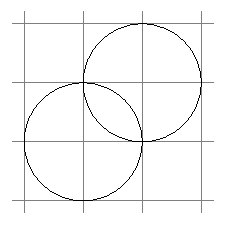
\includegraphics[width=0.5\textwidth]{fig/exam-1213.pdf}
	\caption{Translation invariance}
	\label{fig:translation-invariance}
\end{figure}
\end{solution}
% subsection problem_1 (end)
\subsection{Problem 2} % (fold)
Let \(X_k\) and \(Y_k\) be two random variables whose joint distribution is normal regular distribution on \((\R^2,\B_2)\) with mean \(0\) and variance matrix
\[
	\Sigma_k =
	\begin{pmatrix}
	\frac{1}{k} & 0 \\
	0 & \frac{1}{k}
	\end{pmatrix}
\]
for \(k\in \N\). That is \((X_k,Y_k)^T\sim\mathcal{N}(0,\Sigma_k)\).
\begin{problem}
Show that \(X_k+Y_k\sim\mathcal{N}(0,2/k)\)
\end{problem}
\begin{solution}
Let
\[
    M=\begin{pmatrix}
	   X_k \\
	   Y_k
	   \end{pmatrix},
	\qquad
	\xi = \begin{pmatrix}
	0 \\
	0
	\end{pmatrix},
	\qquad
   B = \begin{pmatrix}
       1 & 1
   \end{pmatrix}
\]
Then using \textbf{Col. 18.29} we get that
\begin{align}
    BM & \sim\mathcal{N}(B\xi,B\Sigma_kB^T) \\
    \begin{pmatrix}
    1 & 1
    \end{pmatrix}
    \begin{pmatrix}
	   X_k \\
	   Y_k
	   \end{pmatrix}&\sim\mathcal{N}\left(
	   \begin{pmatrix}
    1 & 1
    \end{pmatrix}
    \begin{pmatrix}
	0 \\
	0
	\end{pmatrix},
\begin{pmatrix}
       1 & 1
   \end{pmatrix}
   \begin{pmatrix}
	\frac{1}{k} & 0 \\
	0 & \frac{1}{k}
	\end{pmatrix}
	\begin{pmatrix}
	1 \\
	1
	\end{pmatrix}
	\right) \\
    X_k+Y_k &\sim \mathcal{N}(0,2/k)
\end{align}
\end{solution}
\begin{problem}
Show that for all \(\epsilon>0\)
\[
	P\mid X_k+Y_k>\epsilon)\leq\frac{2}{k\epsilon^2}
\]
\end{problem}
\begin{solution}
From Chebychevs inequlity we have that
\[
	P(\mid X-EX\mid > \epsilon) \leq \frac{VX}{\epsilon^2}
\]
Thereby it follows that
\begin{align}
    P(\mid X_k+Y_k-0\mid > \epsilon) &\leq \frac{2/k}{\epsilon^2}\\
     P(\mid X_k+Y_k\mid > \epsilon) &\leq \frac{2}{k\epsilon^2}
\end{align}
Further. Clearly as \(k \rightarrow \infty\), the rhs goes to zero, and thus the probability of \(P(\mid X_k+Y_k-0\mid > \epsilon)\) must also go to zero, by Chebychevs inequality
\end{solution}
% subsection problem_2 (end)
\begin{problem}
Let \(Z=X_2Y_2\). Show that
\[
	EZ=0 \qquad\text{and}\qquad VZ=\frac{1}{4}
\]

\end{problem}
\begin{solution}
We see from \(\Sigma\) that \(X_k,Y_k\) are independent and that \(X_2\sim\mathcal{N}(0,1/2)\) and \(X_2\sim\mathcal{N}(0,1/2)\). So
\[
	E(X_2Y_2)=E(X_2)E(Y_2)=0
\]
Further we see that
\[
	V(X_2Y_2)=E([X_2Y_2]^2)-E(X_2Y_2)^2=E([X_2Y_2]^2)=E(X_2^2)E(Y_2^2)=VX_2VY_2=\frac{1}{4}
\]

\end{solution}
\begin{problem}
Show that
\[
	P\left(\frac{2}{\sqrt{n}} \sum_{i=1}^n Z_i \leq 2 \right)
\]
is convergent for \(n \rightarrow \infty\) and compute the limit.
\end{problem}
\begin{solution}
insert the variance and mean into the CLT formula
\[
	P\left(\frac{1}{\sqrt{n}} \sum_{i=1}^n \frac{Z_i}{1/2} \leq 2 \right)=P\left(\frac{2}{\sqrt{n}} \sum_{i=1}^n Z_i \leq 2 \right) \rightarrow \Phi(2)
\]

\end{solution}
\subsection{Problem 3} % (fold)
\label{sub:problem_3-2012}
For the next question it can be assumed and well known that
\[
	\int^{\infty}_{-\infty}\frac{1}{1+y^2}=\pi
\]
Let \(A(-1,1)\times\R\) and definte the \(\mathcal{M}^+\)-function \(f\) by
\[
	f(x,y)=\indicator{A}(x,y)\frac{\mid x\mid}{2\pi(1+x^2y^2)}
\]
for \((x,y)\in \R^2\)
\begin{problem}
Show that
\[
	\int f\dif m_2=1
\]
\end{problem}
\begin{solution}
\begin{align*}
\int f\dif m_2=\int_{-1}^1\int_{\R}\frac{\mid x\mid}{2\pi(1+x^2y^2)}\dif y\dif x
\end{align*}
Using \textbf{thm 12.7} in ``reverse'' with \(\phi=1/(1+y^2)\) and \(h(y)=xy\) for a fixed \(x\ne 0\) to evaluate the inner integral. It  follows that \(h'(y)=x\), such that
\begin{align}
    \int_\R \phi(h(y))\mid h'(y)\mid &  =\int_{h(\R)}\phi(y)\dif y \\
  \frac{1}{2\pi}\int_\R \frac{1}{1+x^2y^2}\mid x\mid & = \frac{1}{2\pi}\int_\R\frac{1}{1+y^2}=\frac{1}{2}
\end{align}
So
\[
	\int_{(-1,1)\setminus \{0\}}\frac{1}{2}\dif x=\frac{1}{2}x\Big|_{-1}^1=1
\]
where we have used that \(\{0\}\) is a \(m\) null set.
\end{solution}
It \(\mu=f\cdot m_2\), that is, if \(\mu\) is a measure with density \(f\)  w.r.t.\ the Lebeques measure then then it follows from  the question above that \(\mu\) is a probability measure.
\begin{problem}
Show that
\[
	\int x \dif \mu(x,y)=0
\]
\end{problem}
\begin{solution}
first we note from \textbf{thm. 11.7} that
\[
	\int x \dif \mu(x,y)=\int x\cdot f\dif m_2
\]
To check that the function is integrable we note that for \(\mid x\mid \leq1\)
\[
	\int_A \mid x\mid f(x,y)\dif m_2 \leq 	\int_A f(x,y)\dif m_2=1<\infty
\]
So we have that
\[
		\int_A  x f(x,y)\dif m_2=\int_{-1}^1   x \int_{\R}\frac{\mid x\mid}{2\pi(1+x^2y^2)}\dif y\dif x = \int_{-1}^1  \frac{x}{2}\dif x =\frac{1}{4}x^2\Big|_{-1}^1=0
\]

\end{solution}
\begin{problem}
compute the density w.r.t. the Lebesgue measure for the joint distribution of \(X,XY\)
\end{problem}
\begin{solution}
let
\[
	h(x,xy)=
	\begin{pmatrix}
	x \\ xy
	\end{pmatrix}
	=
	\begin{pmatrix}
	z \\
	w
	\end{pmatrix}
\]
which maps \(U:=A\setminus\{(x,y)\mid x=0\}\) bijectivly onto intselfs. We note that \(U\) is open, and that \(h\) and \(h^{-1}\) is \(C^1\) on \(U\).  I then follows that
\[
	h^{-1}(z,w) =
	\begin{pmatrix}
	z \\
	\frac{w}{z}
	\end{pmatrix}
\]
Finding the Jacobian of \(h^{-1}(x,xy)\)
\[
	\Dif h^{-1}(z,w)=
	\begin{pmatrix}
	1 & 0 \\
	-\frac{w}{z^2} & \frac{1}{z}
	\end{pmatrix}
\]
 Thus \(\mid \mathrm{det}\Dif h^{-1}(z,w)\mid=\mid z\mid^{-1}\). Then \(h(\mu)\) has density
 \[
 	\tilde{f}(z,w)=\indicator{U}(z,w)\frac{\mid z\mid}{2\pi(1+w^2)}\mid z\mid^{-1}=\indicator{U}(z,w)\frac{1}{2\pi(1+w^2)}
 \]
\end{solution}
% subsection problem_3 (end)
\section{Problem 4} % (fold)
\label{sec:problem_4 2013}
Let \(\upsilon\) be a measure on \((0,\infty)\) with density
\[
	f(x)=\frac{1}{x^{3/2}}e^{-1/x}, \qquad x>0
\]
w.r.t. the Lebesque measure.
\begin{problem}
Show that
\[
	\upsilon((0,\infty))=\sqrt{\pi}
\]
\textbf{Hint:} Try subsitution with \(h(x)=1/\sqrt{x}\)
\end{problem}
\begin{solution}
We use \textbf{thm. 12.7}. We note that \(h\) is an monotonicly dicreasing function on \((0,\infty)\) and \(h^{-1}(y)=1/y^2\). Thereby maps \((0,\infty)\) to \((0,\infty)\) bijectivly. Further \(h^{-1}\) is \(C^1\) on \((0,\infty)\). Further, the density is 0 on \((0,\infty)^{c}\). We also note that
\[
	h(x)=\frac{1}{\sqrt{x}},\qquad h'(x)=-\frac{1}{2x^{3/2}}
\]
we now note that
\[
	\upsilon((0,\infty))=\int_0^\infty \frac{1}{x^{3/2}}e^{-1/x}\dif x=2\int_0^\infty\exp(-h(x)^2)\mid h'(x)\mid \dif x = \int_0^\infty \exp(-y^2)\dif y=2\cdot\frac{\sqrt{\pi}}{2}
\]
by \textbf{thm 12.7} with \(\phi(x)=\exp(x^2)\)
\end{solution}
By the previus question we can now introduce the probability measure
\[
	\mu=\frac{1}{\sqrt{\pi}}f\cdot m_{(0,\infty)}.
\]
That is, \(\mu\) has density
\[
	g(x)=\frac{1}{\sqrt{\pi}x^{3/2}}e^{-\frac{1}{x}}, \quad x>0
\]
w.r.t. Lebesgue measure. Let \(X\) be  stochastic variable with distribution \(\mu\).
\begin{problem}
Find the density w.r.t. the Lebesgue measure for the distribution of \(1/X\)
\end{problem}
\begin{solution}
We see that \(h(x)=1/x\) which maps \(((0,\infty) )\)  onto \((0,\infty)\) bijectively. Further \(h^{-1}(y)=1/y\) is \(C^1\) on \((0,\infty)\) with \(\left(h(^{-1})\right)'=-1/y^2\).
We the see that
\[
	\tilde{g}(y)=f(h^{-1}(y))\mid (h^{-1})'\mid = \frac{1}{\sqrt{\pi}x^{1/2-1}}e^{-y}
\]
which is the \(\Gamma\)-distribution with shape parameter \(\lambda=1/2\)
\end{solution}
\begin{problem}
Let \(Y\) be another stochastic variable with distribution \(\mu\) such that \(X\) and \(Y\) are independent. Find the distribution of
\[
	\frac{1}{X}+\frac{1}{Y}
\]
\begin{solution}
From \textbf{thm. 18.12} we know that \(1/X\) and \(1/Y\) are independent. By \textbf{ex. 20.11} we have that
\[
	\frac{1}{X}+\frac{1}{Y}
\]
 have density \(\Gamma(1,1)\)
\end{solution}
\end{problem}
% section problem_4 2013 (end)

% section exam_2012_2013 (end)

%%--------------------------------------------------------------------------
%% Reexam 2012/2013
%%--------------------------------------------------------------------------


\section{Reexam 2012/2013} % (fold)
\label{sec:reexam_2012_2013}
\subsection{Problem 1} % (fold)
\label{sub:problem_1}

% subsection problem_1 (end)
\begin{problem}
If \(X\) and \(Y\)  are real valued random variables and \(X\indep Y\), is it then true that \(X^2\indep Y^2\)?
\end{problem}i
\begin{solution}
Yes. \textbf{Thm 18.12:} if \(X\indep Y \Rightarrow h_x(X)\indep h_y(Y)\) with \(h_x=h_y=X^2\)
\end{solution}
\begin{problem}
Let \(X\) be a real valued stochastic variable with \(EX=0\) and such that \(Ee^X<\infty\). Is it true that
\[
	1 \leq Ee^X?
\]
\end{problem}
\begin{solution}
yes: \textbf{Thm 16.31:} From Jensen inequality we have that
\[
	\varphi(EX) \leq E\varphi(X)
\]
Letting \(\varphi(x)=e^x\), we get that
\[
	e^{EX} \leq Ee^X \Rightarrow e^0 \leq Ee^X \Rightarrow 1 \leq Ee^X
\]
\end{solution}
\begin{problem}
Let \(X\) and \(Y\) be independent real valued random variables. Both with exponential distribution with scale paramenter \(\beta=1\). Is it then true that \(X+Y\) is exponentially distributed with scale paramter \(2\)?
\end{problem}
\begin{solution}
No. Let \(Z=X+Y\). The distribution of \(Z\) is then
\[
	f_Z(Z)=\int_{-\infty}^\infty e^{x}e^y = \int_{-\infty}^\infty e^{x+y}
\]
\end{solution}
\begin{problem}
Let \(B=\{(x,y)\in \R^2 \mid x^2+y^2 <\} 1 \}\) and let \(f:[0,\infty) \rightarrow [0,\infty)\) be measurable. Is it true that
\[
	\int_B f(x^2+y^2)\dif m_2(x,y) = 2\pi \int_0^1f(r)r\dif r
\]
\end{problem}
\begin{solution}
From \textbf{Example 12.17}, we see that
\begin{align*}
\int_B f(x^2+y^2)\dif m_2(x,y) & = \int_{(0,2\pi)\times(0,1)}f(r)r \dif m_2(r,\theta) \\
 & = \int_0^{2\pi}\int_0^1 f(r)r \dif r \dif \theta \\
 & = \int_0^{2\pi} \dif \theta \int_0^1 f(r)r \dif r \\
 & = 2\pi\int_0^1 f(r)r \dif r \\
\end{align*}
\end{solution}
\begin{problem}
Is it true that
\[
	F(x)=arctan(x)+\pi/2
\]
is a distribution function on \(\R\)?
\end{problem}
\begin{solution}
\begin{enumerate}
	\item F is clearly increasing as \(d/dx F = 1/(x^2+1) >0\)
	\item F is continus and therby also right continus
	\item \(\lim_{x \rightarrow \infty}F(x)=\pi\)
	\item \(\lim_{x \rightarrow -\infty}F(x)=0\)
\end{enumerate}
As the function \(F(x)\) does not converge to 1, but to \(\pi>1\) F is not a distribution function.
\end{solution}
\subsection{Problem 2} % (fold)
\label{sub:problem_2}
Let \(X\) and \(Y\) be two real valued stochastic variables who's joint distribution is the regular normal distribution on \((\R^2,\B_2)\) with mean 0 and variance matrix
\[
\Sigma =
	\begin{pmatrix}
	\sigma_1^2 & \rho \\
	\rho & \sigma_2^2
	\end{pmatrix}
\]
where we assume that \(\sigma_1^2,\sigma_2^2>0\) and \(-\sigma_1\sigma_2<\rho<\sigma_1\sigma_2\). \(\Sigma\) is positive definite, and can then be a variance matrix for a regular normal distribution.
\begin{problem}
Find the joint distribution of \(X+Y\) and \(X-Y\)
\end{problem}
\begin{solution}
Using \textbf{Col 18.29} with

\[
	B=\begin{pmatrix} 1 & 1 \\ 1 & -1 \end{pmatrix}, \qquad M= \begin{pmatrix} X \\ Y\end{pmatrix} ,\qquad \xi = \begin{pmatrix}
	0 \\ 0\end{pmatrix}
\]
we see that
\[ BM =
	\begin{pmatrix}
	 X + Y \\
	 X - Y
	 \end{pmatrix}
	 \sim\mathcal{N}(B \xi,B\Sigma B^T)=\mathcal{N}(0_{2\times1},
	 \begin{pmatrix}
	  2\sigma_1^2+2\rho & 0 \\
	  0 & 2\sigma_1^2-2\rho
	  \end{pmatrix} )
\]

\end{solution}
\begin{problem}
Determine all values of \(\sigma_1^2,\sigma_2^2\) and \(\rho\) for which \(X+Y\indep X-Y\)
\end{problem}
\begin{solution}
As the \(Cov(X+Y,X-Y)=0\)  we see that \(X+Y\) and \(X-Y\) are always independent.
\end{solution}
\begin{problem}
Assume that \(\sigma_1^2=\sigma_2^2=0.6\) and that \(\rho=0.14\). Find the distribution of
\[
	(X+Y)^2+\frac{1}{0.44}(X-Y)^2
\]
\end{problem}
\begin{solution}
We know that if \(X\sim \mathcal{N}(0,1)\) and all the \(X_i\) are independent, then
\[
	\chi^2=\sum_{i=1}^n X^2_i
\]
is \(\chi^2\) distributed with \(n\)-degrees of freedom. So let's standarize \(X+Y\) and \(X-Y\).
\begin{align}
     \frac{X+Y}{\sigma_1^2+2\rho}&=\frac{X+Y}{2\times0.6^2+2\times 0.14}=X+Y \\
     \frac{1}{0.44}\frac{X-Y}{\sigma_1^2-2\rho}&=\frac{X-Y}{2\times0.6^2-2\times 0.14}=\frac{X-Y}{0.44}0.44=X-Y
 \end{align}
So we conclude that \((X+Y)^2+\frac{1}{0.44}(X-Y)^2\sim\chi^2(2)\)
\end{solution}
% subsection problem_2 (end)
\subsection{Problem 3} % (fold)
\label{sub:problem_3}
Let \(n\in \N\) and consider, for each \(n\), independent real valued stocastic variables \(Z_{1n}\ldots Z_nn\), such that
\[
	P(Z_{nk}=n)=1=1-P(Z_{nk}=0)=\frac{1}{n}
\]
for \(k=1,\ldots,n\). Thus \(Z_{nk}\) takes on almost surly the two values \(n\) and \(0\). Define
\[
 	Y_n=\sum_{i=1}^nZ_{nk}
 \]
 \begin{problem}
 Show that \(EY_n=1\) and that \(VY_n=\frac{n-1}{n} \)
 \end{problem}
\begin{solution}
First we use \textbf{Example 16.20}, and see that \(EZ_{nk}=np=n\frac{1}{n}\)=1. The we use that the expectations of sums is equal to the sums of expectations, so
\[
	EY_n=E \frac{1}{n}\sum_{k=1}^n Z_{nk}=\frac{1}{n}\sum_{k=1}^n EZ_{nk}=\frac{1}{n}n=1
\]
We also see that \(VZ_{nk}=np(1-p)=1-\frac{1}{n}\). Further. Since all the \(Z_nk\)'s are uncorrelated, we have that the variance of the sum, is equal to the sum of the variances.
\[
	VY_n=V \frac{1}{n}\sum_{k=1}^n Z_{nk}=\frac{1}{n}\sum_{k=1}^n VZ_{nk}=\frac{1}{n}n(1-\frac{1}{n})=\frac{n-1}{n}
\]

\end{solution}
\begin{problem}
Consider if \(\sqrt{n}(Y_n-1) \rightarrow \mathcal{N}(0,1)\) \\
\textbf{Hint:} Consider \(P(\sqrt{n}(Y_n-1) \leq1) \)
\end{problem}
\begin{solution}
???
\end{solution}
% subsection problem_3 (end)
\subsection{Problem 4} % (fold)
\label{sub:problem_4}
Define the two \(\mathcal{M^+}\)-functions \(f,g:\R \rightarrow[0,-\infty)\) by \(f(x)=e^x\) and \(g(y)=e^{-y}\). Define two measures \(\mu=f\cdot m\) and \(\upsilon=g\cdot m\)
\begin{problem}
Show that \(\mu\) and \(\upsilon\) are \(\sigma\)-finite
\end{problem}
\begin{solution}
Let
\[
	A_n=[-n,n], \, n\in \N
\]
We note that \(\nsubseti{A}\)

For \(\sigma\)-finiteness, we need to show that
\begin{enumerate}
  	\item \(\mu A_n<\infty\) for all \(n\in\N\)
  	\item \(\bigcup_{n=1}^\infty A_i=\R\)
  \end{enumerate}
(2) follows disrectly from our definition of  \(A_n\). To show (1), we take the integral over the function and show that it is finite.
\begin{align*}
    \mu(A_n) & =\int_{-n}^n f\cdot \dif m=\int_{-n}^n e^x \dif dx = e^x\Big|_{-n}^n =e^n-e^{-n}<\infty \\
      \upsilon(A_n) & =\int_{-n}^n g\cdot \dif m=\int_{-n}^n e^{-y} \dif y = e^{-y}\Big|_{-n}^n =e^{-n}-e^n<\infty
\end{align*}

\end{solution}
By \(\sigma\)-finiteness there is a unique product measure \(\mu\otimes\upsilon\) on \(\R^2,\B_2\)
\begin{problem}
Show that \(\mu\otimes\upsilon\) has density
\[
	(x,y)\mapsto e^{x-y}
\]
w.r.t. \(m_2\) and compute
\[
	A=\mu\otimes\upsilon(\{(x,y)\big| \mid x+y\mid <1,\mid x-y\mid<1\})
\]
\end{problem}
\begin{solution}
Using \textbf{lem 11.5} we get that
\[
	\mu\otimes\upsilon=(f\cdot m)\otimes(g\cdot m)=(f\otimes g)\cdot m_2
\]
where
\[
	(f\otimes g)\cdot m_2(x,y)=(f\otimes g)(x,y)=f(x)g(y)=e^xe^{-y}=e^{x-y}
\]
To find the area on \(A\) define two auxillery sets
\begin{align*}
B &= \{(x,y)\big| -1<x<0,-x-1<y<x+1\} \\
C &= \{(x,y)\big| 0<x<1,x-1<y<-x-1\}\footnote{See \cref{fig:exam-1213}}
\end{align*}
\begin{figure}[htbp]
	\centering
	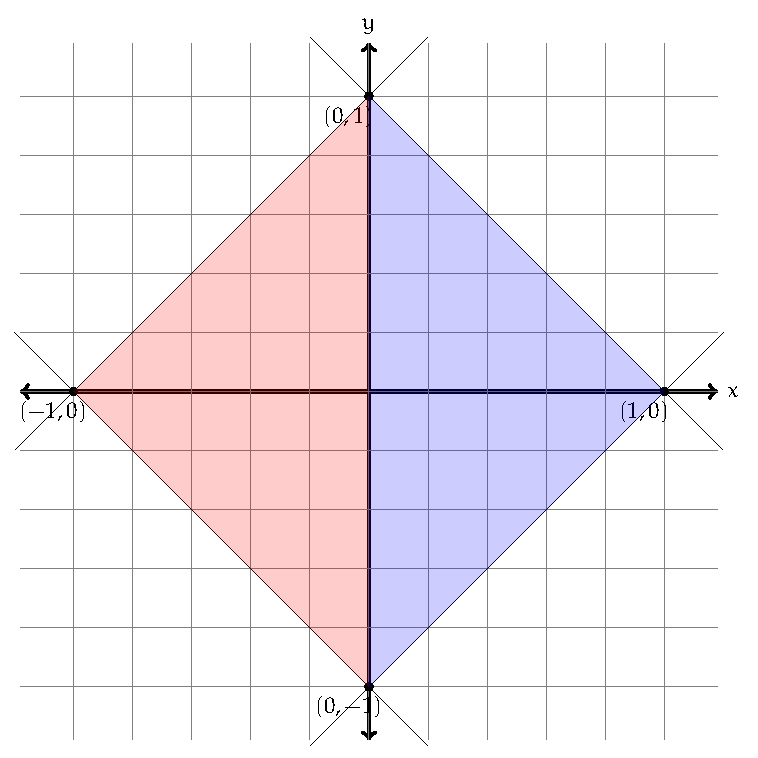
\includegraphics[width=0.7\textwidth]{fig/set-reexam-1213.pdf}
	\caption{\(B\) set in red and \(C\) set in blue. Note that \(C\cup B=A\)  }
	\label{fig:exam-1213}
\end{figure}
Note that
\[
	\indicator{A(x,y)}=\indicator{B\cup C(x,y)}=\indicator{B(x,y)}+\indicator{C(x,y)} = \indicator{(-1,0)}x\indicator{(-x-1,x+1)}y+\indicator{(0,1)}x\indicator{(x-1,-x-1)}y
\]
Using tonelli
\begin{align*}
    & \int_{-1}^0\int_{-x-1}^{x-1}e^{x-y}\dif m_2+\int_0^1\int_{x-1}^{-x+1}e^{x-y} \dif m_2 \qquad \text{ replace the set \(A\) with \(B+C\)} \\
    & \int_{-1}^0e^x\int_{-x-1}^{x-1}e^{-y}\dif x\dif y+\int_0^1e^x\int_{x-1}^{-x+1}e^{-y} \dif x\dif y \qquad \text{ Use Tonellie} \\
    & \int_0^1e^x \left(-e^{-x+1}+e^{x-1}\right) \dif x+\int_0^1e^x\left(-e^{x+1}+e^{-x+1}\right) \dif x \qquad \text{ Evaluate the inner integral} \\
    & \int_0^1 -e^{-1}+e^{2x+1} \dif x+\int_0^1e^x -e^{2x+1}+e^1 \dif x \qquad \text{ Rearrange} \\
    & e\cdot\int_0^1e^{2x} \dif x -e^{-1}+e-e^{-1}\cdot\int_0^1-e^{2x} \dif x \qquad \text{ Rearrange} \\
    & e \frac{1-e^{-2}}{2}-e^-1+e-e^-1 \frac{e^2-1}{2} \\
    & \frac{e}{2}- \frac{e^{-1}}{2} -e^{-1}+e \frac{e}{2}+\frac{e^{-1}}{2}=e+e^{-1}
\end{align*}
\end{solution}
\begin{problem}
Let \(h(x, y) = \indicator{A}(x, y)xy\) with \(A = (-\infty, 0) \times (0, \infty)\). Compute
\[
	\int h\dif \mu\otimes \upsilon
\]
\end{problem}
\begin{solution}
First note that \(h\) is a function defined on a negative set \(A\). So \(h\) is a negative function. Define a new function \(g\coloneqq-h\in \mathcal{M}^+\).
\begin{figure}[htbp]
	\centering
	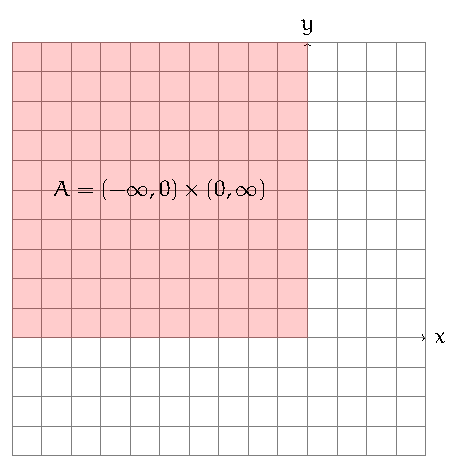
\includegraphics[width=0.5\textwidth]{fig/set-reexam-1213-2.pdf}
	\caption{The set \(A = (-\infty, 0) \times (0, \infty)\)}
	\label{fig:exam-1213-2}
\end{figure}
\begin{align*}
    \int g \dif (\mu\otimes\upsilon) & = \int g(x,y)e^{x-y}\dif m_2(x,y) \\
    & =\int \int -\indicator{A}(x,y)xye^{x-y}\dif x\dif y \\
    & = \int_0^\infty \int_{-\infty}^0 -xye^{x-y}\dif x\dif y \\
    & = \int_0^\infty -xe^x \dif x\int_{-\infty}^0 ye^{-y}\dif y \\
    & = \int_{-\infty}^0 xe^x \dif x\int_0^\infty -ye^{-y}\dif y \\
    & = \left(\int_0^\infty -ye^{-y}\dif y\right)^2 \\
    & = \left(\left[-y(-e^{-y})\right]_0^\infty+\int_0^\infty e^{-y}\right)^2 \\
    & = \left( \left[-e^{-y}\right]_0^\infty \right)^2 \\
    & = 1
\end{align*}
So \(g=\mid h\mid\) is \(h\)-integrable w.r.t \(\mu\otimes\upsilon\) and
\[
	\int h\dif (\mu\otimes\upsilon)=-\int g \dif \mu\otimes\upsilon=-1
\]

\end{solution}
% subsection problem_4 (end)
\subsection{Problem 5} % (fold)
\label{sub:problem_5}
Let \(X,Y\) and \(Z\) be three indenependent real valued random variables. Al with finite second momennt and all with mean \(0\) and variance \(1\). Define
\[
	W= \frac{X+YZ}{\sqrt{1+Z^2}}
\]
\begin{problem}
Show that \(V(W\mid Z)=1\) a.e.
\end{problem}
\begin{solution}
We have that
\begin{align}
    V(W\mid Z) & = \frac{V(X+YZ\mid Z)}{1+Z^2} \\
    V(X+YZ\mid Z) & =  V(X\mid Z)+ V(YZ\mid Z) = V(X) + Z^2V(Y)=1+Z^2
\end{align}
\end{solution}
\begin{problem}
Find the distribution of \(W\) under the additional assumption that \(X,Y\) and \(Z\) all have a marginal \(\mathcal{N}(0,1)\)-distribution

\textbf{Hint:} Compute \(P(W \leq w )\) by Tonellie, intergrating out of the joint distribution of \((X,Y)\) first.
\end{problem}
\begin{solution}
\begin{framed}
For independent \(T_1\sim\mathcal{N}(\mu_{T_1} , \sigma_{T_1}^2)\) and \(T_2\sim\mathcal{N}(\mu_{T_2} , \sigma_{T_2}^2)\)  we have
\begin{align}
    \Phi\left(\dfrac{\mu_{T_2}-\mu_{T_1}}{\sqrt{\sigma_{T_1}^2{}+{}\sigma_{T_2}^2}}\right){}={}P\left(T_1<T_2\right){}={}\displaystyle\dfrac{1}{\sigma_{T_2}\sqrt{2\pi}}\int\limits_{{-}\infty}^{\infty}{}\Phi\left(\dfrac{t-\mu_{T_1}}{\sigma_{T_1}}\right)e^{-\frac{1}{2}\left(t-\mu_{T_2}\right)^2/\sigma^2_{T_2}}\,\,\mathrm dt\,,
\end{align}
where \(\Phi\)  is the CDF for the standard normal distribution
\end{framed}
So, after using the definition of conditional probability, the independence of \(x\)  and \(\left\{Y, Z\right\}\)  and Tonelli's theorem (to justify the iterated integrals and ``associativity'' thereof), we can use the observation above to solve the integral as follows:
\begin{align*}
P\left(W<w\right)&=P\left(\dfrac{X+YZ}{\sqrt{1+Z^2}}<w\right)=P\left(X+YZ<w\sqrt{1+Z^2}\right)\\
&=P\left(X<w\sqrt{1+Z^2}-YZ\right)\\
&=\dfrac{1}{\left(\sqrt{2\pi}\right)^2}\int\limits^{\infty}_{{-}\infty}\int\limits^{\infty}_{{-}\infty} P\left(X<w\sqrt{1+z^2}-yz\,\bigg|\,\,Y=y,Z=z\right)e^{-\frac{1}{2}\left(y^2+z^2\right)}\mathrm dy\,\mathrm dz\\
&=\dfrac{1}{\left(\sqrt{2\pi}\right)^2}\int\limits^{\infty}_{{-}\infty}\int\limits^{\infty}_{{-}\infty} P\left(X<w\sqrt{1+z^2}-yz\right)e^{-\frac{1}{2}\left(y^2+z^2\right)}\mathrm dy\,\mathrm dz\\
&=\dfrac{1}{\left(\sqrt{2\pi}\right)^2}\int\limits^{\infty}_{{-}\infty}\left(\,\,\,\int\limits^{\infty}_{{-}\infty} P\left(X<w\sqrt{1+z^2}-yz\right)e^{-\frac{1}{2}y^2}\mathrm dy\right)e^{-\frac{1}{2}z^2}\,\mathrm dz\\
&=\dfrac{1}{\left(\sqrt{2\pi}\right)^2}\int\limits^{\infty}_{{-}\infty}\left(\,\,\,\int\limits^{\infty}_{{-}\infty} \Phi\left(w\sqrt{1+z^2}-yz\right)e^{-\frac{1}{2}y^2}\mathrm dy\right)e^{-\frac{1}{2}z^2}\,\mathrm dz\\
&=\dfrac{1}{\sqrt{2\pi}}\int\limits^{\infty}_{{-}\infty}\dfrac{1}{z\sqrt{2\pi}}\left(\,\,\,\int\limits^{\infty}_{{-}\infty} \Phi\left(u\right)e^{-\frac{1}{2}\left(u-w\sqrt{1+z^2}\right)^2/z^2}\mathrm dy\right)e^{-\frac{1}{2}z^2}\,\mathrm dz\\
&=\dfrac{1}{\sqrt{2\pi}}\int\limits^{\infty}_{{-}\infty} \Phi\left(w\right)e^{-\frac{1}{2}z^2}\,\mathrm dz\\
&=\Phi\left(w\right)\,
\end{align*}
Therefore, \(W\sim\mathcal{N}\left(0,1\right)\) .
\end{solution}
% subsection problem_5 (end)
% section reexam_2012_2013 (end)

\section{Exam 2013/2014} % (fold)
\label{sec:exam_2013_2014}
\subsection{Problem 1} % (fold)
\begin{problem}
Let \(X\sim\mathcal{N}(0,1)\).  Argue that the distribution for \(\exp(X)\) has density w.r.t. the Lebesgue measure. You do not need to find the density.
\end{problem}
\begin{solution}
From \textbf{thm. 15.1} we know that the distribution has density as
\begin{enumerate}
	\item h maps \(\R\) onto \(\R^+\)
	\item \(h^{-1}=\log(x)\) is \(C^1\)  on \(\R^+\)
	\item \(P(X\in \R)=1\)
\end{enumerate}
\end{solution}
\begin{problem}
Assume that
\[
	\begin{pmatrix}
	X_1 \\ X_2
	\end{pmatrix}
	\sim \mathcal{N}\left(
	\begin{pmatrix}
	0 \\0
	\end{pmatrix},
	\begin{pmatrix}
	2 & 0 \\
	0 & 2
	\end{pmatrix}
	\right)
\]
Determine if \(X_1\indep X_2\).
\end{problem}
\begin{solution}
As the joint distribution of \(X_1\) and \(X_2\) has \(Cov(X_1,X_2)=0\), it follows from \textbf{thm. 18.27} that \(X_1\indep X_2\).
\end{solution}
\begin{problem}
Assume that \(X_1\ldots X_n\) are iid. with
\[
	P(X_i=2)=P(X_i=-2)=\frac{1}{2}
\]
Determine if
\[
	P\left(\sum_{i=1}^n X_i \leq 2x\sqrt{n}\right) \rightarrow\Phi(x)
\]
for \(n \rightarrow\infty\)
\end{problem}
\begin{solution}
As \(X_i\)'s are bounded by \(\{-2,2\}\) all moments exists. \(EX=-2\frac{1}{2}+2\frac{1}{2}=0\) and \(VX=(-2)^2\frac{1}{2}+2^2\frac{1}{2}=4\), so \(\sigma=\sqrt{4}=2\). It the follows from the CLT that
\[
	P\left(\sum_{i=1}^n X_i \leq 2x\sqrt{n}\right) = P\left(\frac{1}{\sqrt{n}}\sum_{i=1}^n \frac{X_i}{2}\leq x\right)\rightarrow\Phi(x)
\]

\end{solution}
% subsection problem_1 (end)
\subsection{Problem 2} % (fold)
Assume that \(X\) and \(Y\) are independent real valued random variables  and that \(X\) is uniformly distributed on \((-1,1)\) and that \(Y\) is \(\Gamma\)-distributed with shape parameter \(\lambda=3\)
\begin{problem}
Show  that
\[
	E\left(\frac{1}{Y}\right)=\frac{1}{2}
\]
\end{problem}
\begin{solution}
Use \textbf{Thm. 15.1} with \(h=1/Y\). We see that \(h\) and  \(h^{-1}=1/X\)  is a monotonically decreasing function on \((0,\infty)\) and thereby also bijective. Further we follows that \(P(Y\in (0,\infty))=1\). Thereby we can apply the theorem. So
\begin{align}
    f\left(h^{-1}\left(\frac{1}{y}\right)\right)\left| \left(h^{-1}\right)'\left(\frac{1}{y}\right)\right|&=\frac{1}{2}\left(\frac{1}{x}\right)^{2}e^{-1/x}\left(\frac{1}{x^2}\right)\\
    & = \frac{1}{2}\frac{1}{x^4}e^{\rfrac{1}{-x}}
\end{align}
so the distribution of \(1/Y\) is
\[
	\tilde{f}=\left\{
	\begin{matrix}
	 \frac{1}{2}\frac{1}{x^4}e^{\rfrac{1}{-x}} & \text{ for } x\in(0,\infty) \\
	 0 & \text{ for } x\notin (0,\infty)
	 \end{matrix} \right.
\]

Calculating the expectation
\begin{align*}
    	\int_0^{-\infty}x\cdot\frac{1}{2}\frac{1}{x^4}e^{\rfrac{1}{-x}}\dif x & =\int_0^{-\infty}\frac{1}{2}\frac{1}{x^3}e^{\rfrac{1}{-x}}\dif x & \\
    	& = \frac{1}{2}\int_0^{-\infty}\frac{1}{x^3}e^{\rfrac{1}{-x}} \dif x& \text{Factor out the constant} \\
    	&= \frac{1}{2}\int_0^{-\infty}ue^{-u} \dif u& \text{change \(u=\rfrac{1}{x}\) } \\
    	& = \frac{1}{2}\underbrace{\left[ue^{-u}\right]_0^\infty}_{=0}-\frac{1}{2}\int_0^\infty e^{-u} \dif u & \text{integration by parts} \\
    	& =-\frac{1}{2}\left[-e^{-u}\right]_0^\infty & \text{evaluate the integral} \\
    	& =-\frac{1}{2}\left[-e^{-\rfrac{1}{x}}\right]_0^\infty & \text{revert} \\
    	& = \frac{1}{2}
\end{align*}
\begin{framed}
A faster way is to use \textbf{Example 16.6}. Let \(t(x)\) be a transformation, then
\[
	Et(x)=\int t(h\dif \mu)
\]
So with \(t(x)=\rfrac{1}{y}\) and \(f\mu=\int \frac{1}{2}x^2e^{-x}\)  we get that
\begin{align}
	\int_{-\infty}^\infty\indicator{(0,\infty)}\frac{1}{y}\frac{1}{2}y^2e^{-y}\dif y  & = \int_{0}^\infty\frac{1}{2}ye^{-y}\dif y \\
	& = \frac{1}{2} \underbrace{\int_{0}^\infty ye^{-y}\dif y}_{\text{Exponential density}} \\
	& = \frac{1}{2}\cdot 1=\frac{1}{2}
\end{align}

\end{framed}
\begin{problem}
Compute
\[
	\expect*{\frac{X}{Y}| X} \text{ ans show that } \expect*{\frac{X}{Y}}=0
\]
\end{problem}
\begin{solution}
As \(X\indep Y\) we have that
\[
	\expect*{\frac{X}{Y}| X}=\expect*{ X| X}\expect*{\frac{1}{Y}| X}=X\expect*{\frac{1}{Y}}=0\frac{1}{2}=0
\]

\end{solution}
\end{solution}
% subsection problem_2 (end)
\subsection{Problem 3} % (fold)
\label{sub:problem_3 2013}
Define the function \(F:\R \rightarrow[0,\infty)\) by
\[
	F(x)=1-\frac{1}{1+\log(x+1)}
\]
for \(x\geq0\) and \(F(x)=0\) for \(x<0\). It can be used, without proof that \(F\) is a distribution function for a measure on \((\R,\B)\). Let \(\upsilon\) be a probability measure with distribution function \(F\). That is
\[
	F(x)=\upsilon((-\infty,x])
\]
\begin{problem}
Draw a graph of the distribution function \(F\). Explain that \(\upsilon\) has density w.r.t. the  Lebesgue measure and find the density.
\end{problem}
\begin{solution}
\begin{figure}[htbp]
	\centering
	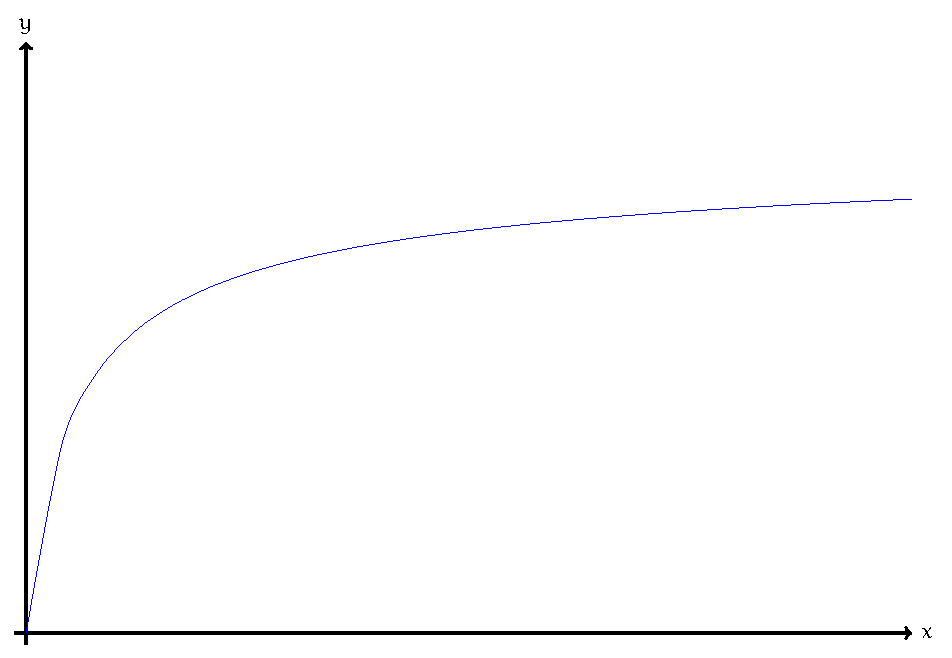
\includegraphics[width=0.95\textwidth]{fig/exam-2013.pdf}
	\caption{Plot of \(\displaystyle F(x)=1-\frac{1}{1+\log(x+1)}\) }
\end{figure}
We further note that \(F\) is \(C^1\) on \([0,\infty)\) with
\[
	f(x)=F'(x)=\frac{1}{(1+\log(x+1))^2(x+1)}
\]
We see that
\[
	\int_0^\infty f(x)=F(x)\Big|_0^\infty = 1
\]
We thereby conclude that \(\upsilon\) has density
\[
	f(x)=\left\{
	\begin{matrix}
	\frac{1}{(1+\log(x+1))^2(x+1)} &  \text{for } x>0 \\
	0 &  \text{for } x\leq0
	\end{matrix}
	\right.
\]
w.r.t. the Lebesgue measure.
\end{solution}
% subsection problem_3 2013 (end)
% section exam_2013_2014 (end)